\chapter{MC-SBD-STM Performance}

\section{Synthetic Data Generation Process}
We also used a new approach in selecting kernel size. In the original model, kernel size was artificially assigned as free parameter; However, we believe the kernel size should represent the natural span of the QPI pattern, where its cutoff is determined by the noise level. We illustrate the process in Figure. \ref{fig:ch7_kernel_size}, 

\begin{figure}
	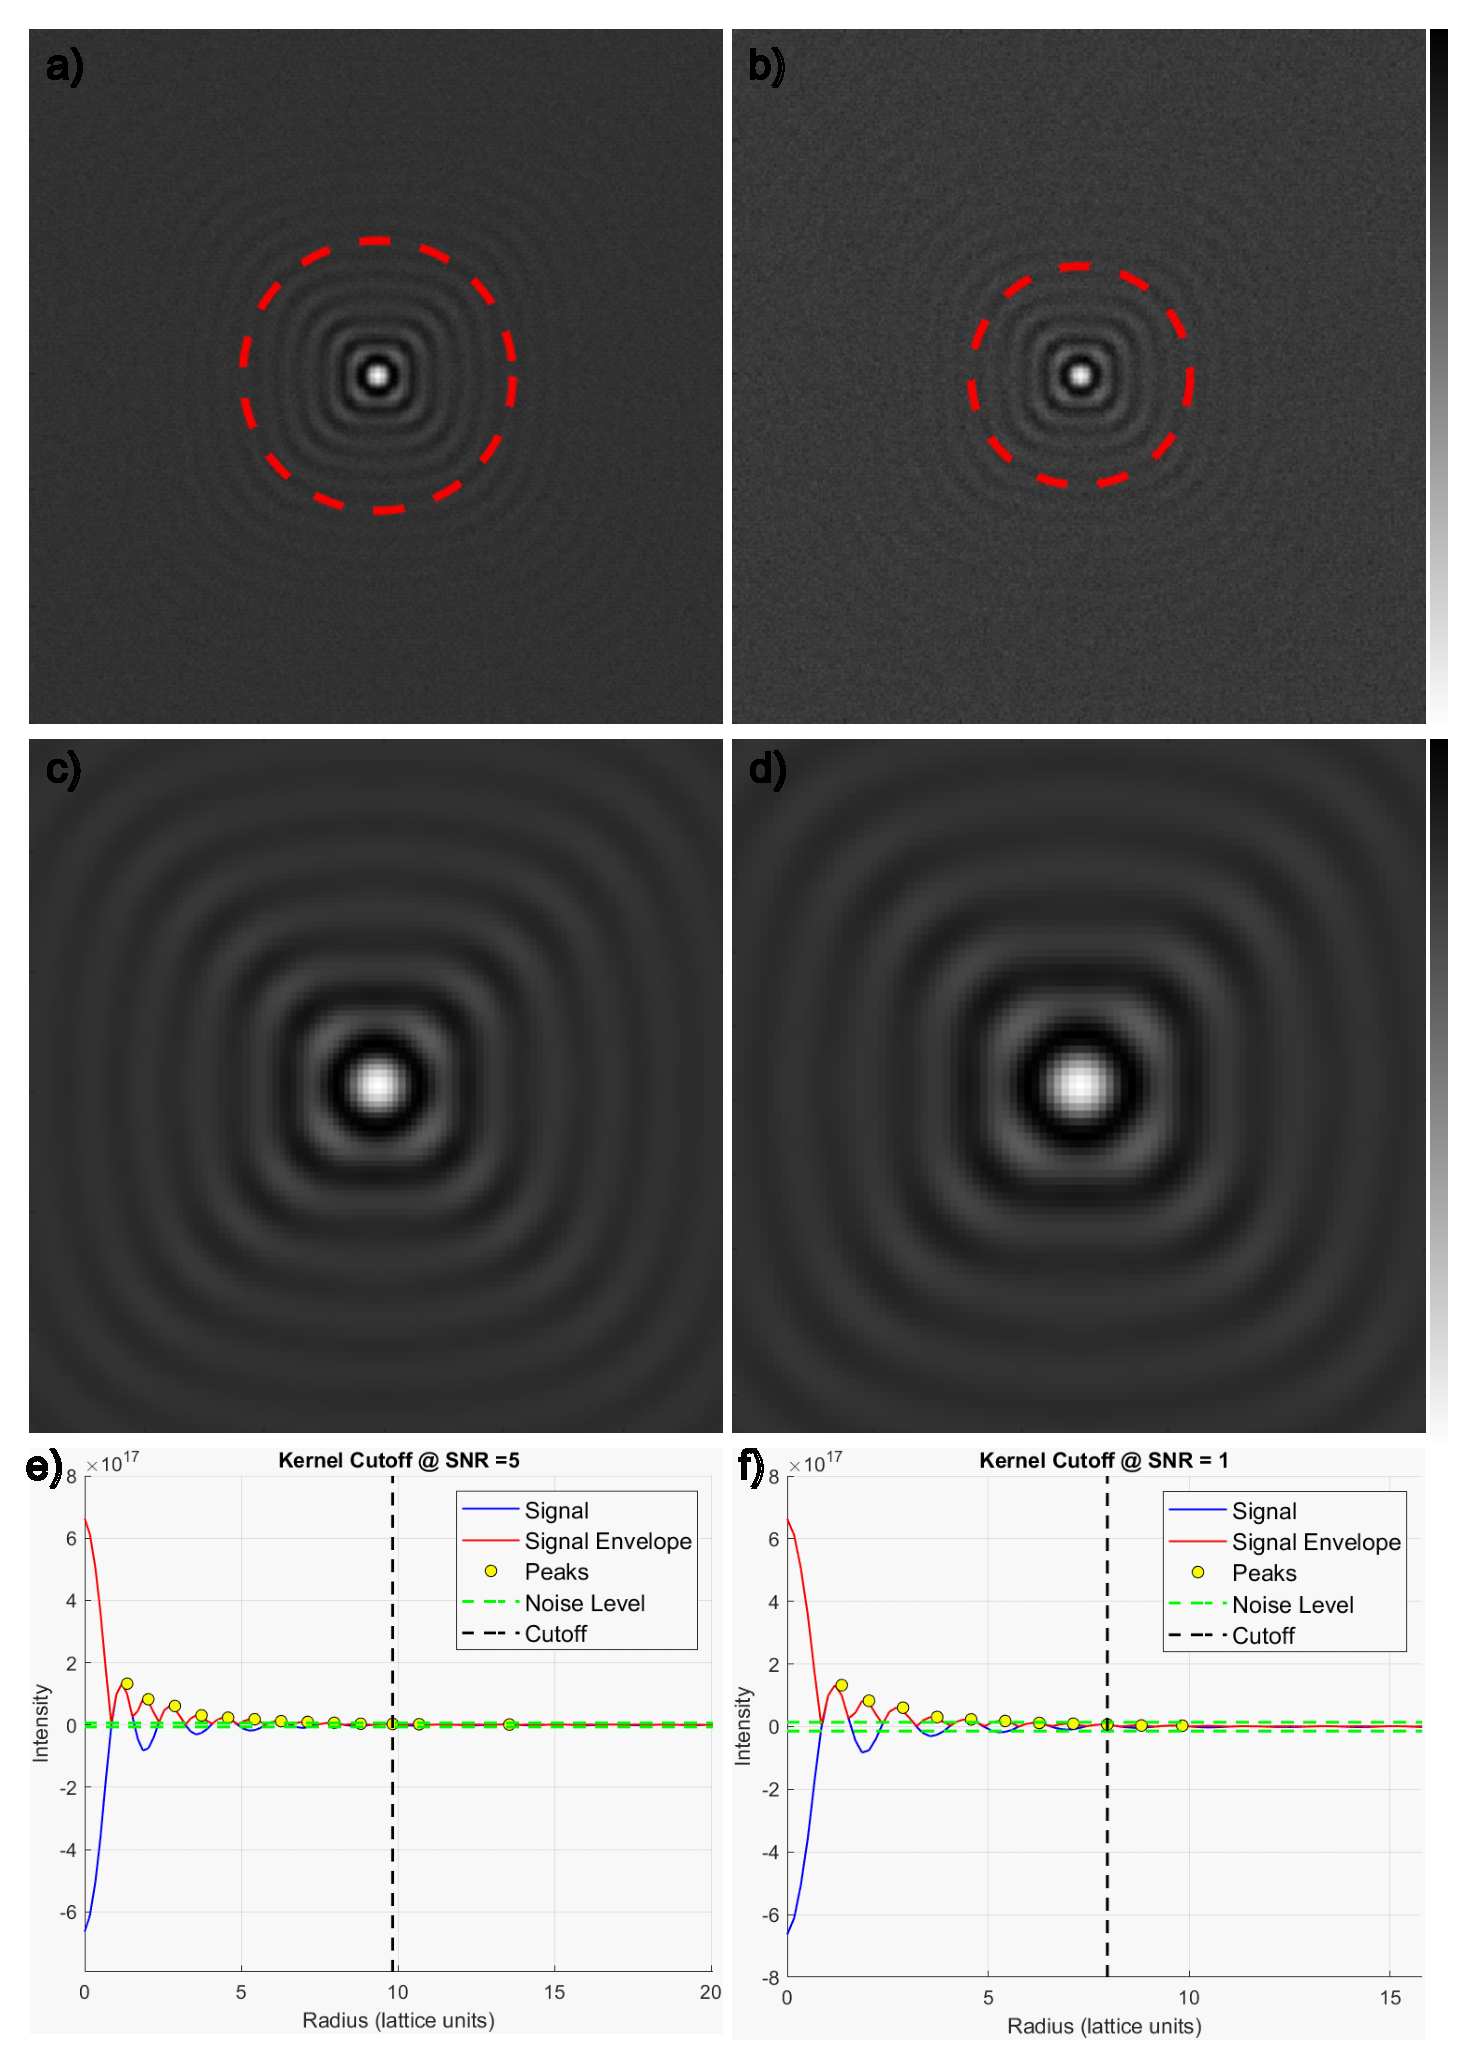
\includegraphics[width= \textwidth]{kernel_size.pdf} 
	\centering
	\caption{}
	\label{fig:ch7_kernel_size}
\end{figure}
\subsection{Tune-able parameter space}

\section{Benchmark tests on the parameter space}
\subsection{sparsity}
\subsection{Number of defect types}
\subsection{spatial resolution and noise level}

\section{MC-SBD-STM on real data}
\subsection{real data complexity}
\subsection{preprocessing pipelines}
\subsection{Result on ZrSiTe}
\subsection{Potential use in other materials}
